\documentclass[12pt]{book}

\usepackage[dvips,letterpaper,margin=0.75in,bottom=0.5in]{geometry}
\usepackage{cite}
\usepackage{slashed}
\usepackage{graphicx}
\usepackage{amsmath}
\usepackage{amssymb}
\usepackage{braket}
\usepackage{pythonhighlight}
\begin{document}

\newcommand{\ihbar}{\ensuremath{i \hbar}}
\newcommand{\Pss}{\ensuremath{\Psi^*}}
\newcommand{\dPsidt}{\ensuremath{ \frac{\partial \Psi}{\partial t} }}
\newcommand{\dPsidx}{\ensuremath{ \frac{\partial \Psi}{\partial x} }}
\newcommand{\ddPsidx}{\ensuremath{ \frac{\partial^2 \Psi}{\partial x^2} }}
\newcommand{\dPssdt}{\ensuremath{ \frac{\partial \Psi^*}{\partial t} }}
\newcommand{\dPssdx}{\ensuremath{ \frac{\partial \Psi^*}{\partial x} }}
\newcommand{\ddPssdx}{\ensuremath{ \frac{\partial^2 \Psi^*}{\partial x^2} }}

\newcommand{\dphidt}{\ensuremath{ \frac{d \phi}{dt} }}
\newcommand{\dpsidx}{\ensuremath{ \frac{d \psi}{dx} }}
\newcommand{\ddpsidx}{\ensuremath{ \frac{d^2 \psi}{dx^2} }}


\title{PHY 115L \\ Finite Square Well}
\author{Michael Mulhearn}

\maketitle

\setcounter{chapter}{0}
\chapter{Time-Independent Schr\"odinger Equation}

In the previous homework, we numerically integrated the Time-Independent Schr\"odinger Equation (TISE):
\begin{equation}
- \frac{\hbar^2}{2 m} \; \ddpsidx \, + \, V(x) \, \psi(x) = E \, \psi(x)\\
\end{equation}
using the Fourth-Order Runge-Kutta technique.  We adopted a system of units based on a characteristic length scale $a$ and energy $E_0$ with
\begin{equation}
E_0 \equiv \frac{\hbar^2}{2ma^2}
\end{equation}
In our computer programs, we'll measure $x$ in units of $a$ and $E$ in units of $E_0$.  In these units $a=1$ and $E_0=1$.

\section{Bound States of the Finite Square Well}

Next we consider the finite square well potential:
$$\frac{V(x)}{E_0} = \begin{cases}
-z_0^2, & -a \leq x \leq a \\
0     & {\rm otherwise} \\
\end{cases}
$$
Where $z_0^2$ is a dimensionless constant, nicely consistent with our system of units, that sets the depth of the well (in units of $E_0$). As the potential is finite everywhere, we expect both $\psi$ and $d\psi/dx$ to be continuous.
The bound state potentials will have 
$$-z_0^2 < \frac{E}{E_0} < 0.$$
For $x < -a$ and $x > a$, the TISE becomes (using our system of units):
\begin{equation*}
a^2 \frac{d^2 \psi}{d x^2} = -\frac{E}{E_0}\psi(x) = 
(\kappa a)^2 \psi(x), \hspace{2cm} \kappa \equiv \frac{1}{a} \; \sqrt{\frac{-E}{E_0}}.
\end{equation*}
with the solutions
$$\psi(x) = A e^{\displaystyle \kappa x}$$
for $x<-a$ and
$$\psi(x) = B e^{\displaystyle -\kappa x}$$
for $x>a$.  Within the potential well at $-a \leq x \leq a$ we have:
\begin{equation*}
a^2 \frac{d^2 \psi}{d x^2} = -\left(z_0^2+\frac{E}{E_0}\right)\psi(x) = -k^2 \psi(x), \hspace{2cm} k \equiv \frac{1}{a}\sqrt{z_0^2+\frac{E}{E_0}}.
\end{equation*}
with general solution:
$$\psi(x) = C \sin(kx) + D \cos(kx)$$
At this point, we will save ourselves a lot of hassle by noting that $V(x)$ is even, and so the general solutions can be constructed as either even or odd solutions\footnote{See Griffith's P2.1c.  Or note that if $\psi(x)$ is a solution, so is $\psi(-x)$, and we can add or subtract the two to get even and odd solutions.}  So we need only establish continuity for $x \geq 0$ and we will automatically have it for $x \leq 0$.

Starting with the even solutions and $x\geq0$, we write:
$$\psi(x) = \begin{cases}
Be^{\displaystyle -\kappa x} & x > a \\
D \cos(kx) & 0 \leq x \leq a \\
\end{cases}$$
and continuity implies:
\begin{equation}
\label{eqn:fswcont}
B e^{-\kappa a} = D \cos(ka)
\end{equation}
We see that the dimensionless quantities $\kappa a$ and $ka$ are of interest, so it will simplify things to note that:
$$(ka)^2+(\kappa a)^2 = z_0^2$$
The derivative is:
$$\frac{d\psi}{dx} = \begin{cases}
-\kappa \, B \, e^{\displaystyle -\kappa x} & x > a \\
-kD \sin(kx) & 0 \leq x \leq a \\
\end{cases}$$
which both must be continuous at $x=a$, so:
\begin{eqnarray*}
-\kappa B e^{-\kappa a} &=& -k D \sin(ka)\\
 \kappa B e^{-\kappa a} &=& k D \sin(ka)\\
 (\kappa a) B e^{-\kappa a} &=& (ka) D \sin(ka)\\
\end{eqnarray*}
where we have multiplied by $a$ so that the equation is in terms of the dimensionless constants $ka$ and $\kappa a$.  Dividing by Equation~\ref{eqn:fswcont} we obtain:
\begin{eqnarray*}
\kappa a &=& (ka) \, \tan(ka) \\
\sqrt{z_0^2-(ka)^2} &=& (ka) \, \tan(ka) \\
\sqrt{z_0^2-z^2} &=& z \, \tan(z) \\
\end{eqnarray*}
where we have defined 
$$z \equiv ka = \sqrt{z_0^2 + \frac{E}{E_0}}$$
and so finally:
\begin{equation}
\sqrt{\left(\frac{z_0}{z}\right)^2-1} = \tan(z) 
\end{equation}
This is an equation with no known algebraic solution.  It can be solved graphically or numerically.  See Fig.~\ref{fig:finitewell}.
\begin{figure}[thb]
\begin{center}
{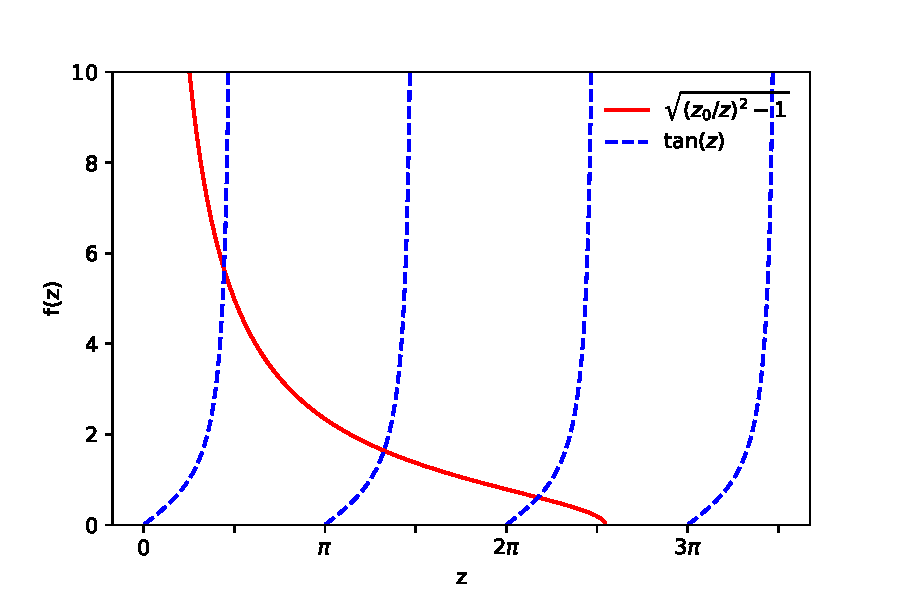
\includegraphics[width=0.60\textwidth]{plots/finitewell.pdf}}
\end{center}
\caption{\label{fig:finitewell} The allowed energies for the finite potential occur at the intersection of these curves.}
\end{figure}
There are some interesting limiting cases to consider.  When:
$$z_0 < \frac{\pi}{2}$$
there is only one bound state (we haven't found the odd solutions yet, which is why this is $\pi/2$ and not $\pi$, as you might expect from the figure...)  Recalling the definition for $z_0$, this amounts to:
$$V_0\,a^2 < \frac{\pi^2 \hbar^2}{8m}$$
which defines a shallow and narrow well.

Alternative, if $z_0$ is very large, then the intersection points are at:
$$z = \frac{n\pi}{2}, \hspace{2cm} n=1,3,5,\ldots$$
which means the allowed energies are:
$$E + V_0 = \frac{n^2\pi^2\hbar^2}{2m(2a)^2}$$
which (relative to the bottom of the well) are the energies of the infinite square well.

\section{Homework Problems}

\noindent
{\bf Problem 1:}  The allowed energies for even solutions of the finite square well potential can be determined by finding the roots of the equation:
$$f_{\rm even}(z) = \sqrt{z_0^2-z^2} \; - \; \tan(z)$$

\noindent
(A) For $z_0 = \pi/2$ find the root of the $f_{\rm even}$ and compute the corresponding allowed energy.  This is the only allowed energy for this narrow and shallow well.\\[5pt]

\noindent
(B) Determine the equation $f_{\rm odd}(z)$ corresponding to odd solutions.\\[5pt]

\noindent
(C) For $z_0 = \pi$, find one root of $f_{\rm even}$ and one root of $f_{\rm odd}$, and compute the corresponding allowed energies (in units of $E_0$).\\[5pt]

\noindent
(D) For $z_0 = 3\pi$, find all allowed energies for even and odd solutions.\\[5pt]

\noindent
(E) Show that for large $z_0$, the first four allowed energies correspond to a kinetic energy:
$$K/E_0 = E + z_0^2$$
which approaches the first four allowed energies of the infinite square well potential.  Hint:  these corresponding to roots
$$z = \frac{n \pi}{2} \hspace{2cm} n=1,2,3,4.$$\\[5pt]

\noindent
{\bf Problem 2:} Use your RK-4 numerical integration to find the even and odd solutions for $z^0 = \pi$.  Compare to your results to the results of Problem 1, and plot the normalized wave functions.\\[5pt]

\noindent
{\bf Problem 3:}  In this problem, you will model two finite square wells of width $2a$ with $z_0=\pi/2$ separated by a small distance $2 \delta a$ where $\delta$ is a small dimensionless quantity.\\[5pt]

\noindent
(A) Use your RK-4 numerical integration to find an even solution for $\delta=0.1$.  Hint: the allowed energy will be near your solution to 1A.  Plot the results.\\[5pt]

\noindent
(B) Use your RK-4 numerical integration to find an odd solution for $\delta=0.1$.  Hint: the allowed energy will be near your solution to 1A.  Plot the results.  (Are you surprised you now have two solutions?)\\[5pt]

\noindent
(C) The difference between the energy of the even solution and your answer to Problem 1A can be though of as a bonding energy.  Plot the bonding as a function of $\delta$.\\[5pt]


\end{document}

